\documentclass[a4paper,12pt]{report}

\usepackage{graphicx} % Required for inserting images
\usepackage{geometry} % To control page margin and size
\usepackage[hidelinks % To hide red boxes around hyperlinks
, pdfborder={0 0 0}]{hyperref} % To add hiperlinks and hrefs to pdf
\usepackage{fancyhdr} % Custom Headers and Footers
\usepackage{listings} % To be abale to add source code
\usepackage{minted}   % For JSON
\usepackage{caption}  % To customize captions 
\usepackage[main=english,ukrainian]{babel} % To customize captions 
\usepackage[utf8]{inputenc} % for urkainian encoding
\usepackage[autostyle=true]{csquotes} % Something with quotations style
\usepackage{setspace} % Spacing
\usepackage[backend=biber,style=numeric-comp,natbib=true,sorting=none,maxnames=4,giveninits=true]{biblatex} % For citations
\usepackage{float} % To use H in table placement
\usepackage{xcolor} % Required for specifying custom colours
\usepackage{booktabs} % For professional rules (toprule, midrule)
\usepackage{array}    % For better column text wrapping
% BIBLIOGRAPHY
\addbibresource{bibliography.bib} % The filename of the bibliography

% LAYOUT SETTINGS
\geometry{a4paper, margin=2.5cm}
\onehalfspacing

\hypersetup{
    colorlinks=true,
    linkcolor=blue,
    citecolor=blue,
}
% HEADERS AND FOOTERS SETTING
\pagestyle{fancy}
\fancyhf{} % Clear existing header and footer
\fancyhead[R]{\thepage} % Page number on the top right
\fancyhead[L]{\leftmark} % Chapter title on the top left
\setlength{\headheight}{15pt}
\fancypagestyle{plain}{
    \fancyhf{} % Cleare default header and footer
    \fancyhead[R]{\thepage} % Page number on the top right
    \renewcommand{\headrulewidth}{0pt} % When it is beginning of the chapter - be without headline
}

% TABLE OF CONTENTS SETTING
\addto\captionsenglish{\renewcommand{\contentsname}{Table of Contents}}

% SETUP
\AtBeginDocument{
    % For title page
\newcommand{\thesistitle}{Development of data pipeline for processing of streaming data on a cloud platform}
\newcommand{\suptitle}{Senior Lecturer}
\newcommand{\supname}{Dmytro \textsc{Cherkasov}}
\newcommand{\specialty}{\enquote{Software Engineering} - F3}
\newcommand{\authorname}{Volodymyr \textsc{Materynskyi}}
\newcommand{\university}{National University of \enquote{Kyiv-Mohyla Academy}}
\newcommand{\department}{Department of Informatics}
\newcommand{\faculty}{Faculty of Informatics}
\newcommand{\thesisdate}{April 2026}
\newcommand{\mon}{Ministry of Education and Science of Ukraine}
\newcommand{\thesisyear}{2026}

% For individual task page
\newcommand{\PMcontents}{
Abstract\\
Introduction\\
Related work\\
Approach\\
Solution\\
Evaluation\\
Further work and Conclusions\\
Bibliography
}
    \hypersetup{
        pdftitle={\thesistitle},
        pdfauthor={\authorname} 
    }
}

\begin{document}
\pagenumbering{roman} % Use roman numerals for page numbering

% Preliminaries pages
\begin{titlepage}
\doublespacing
    \begin{center}
        \centering
        \large{\mon}\\
        \textbf{\university}\\
        \department \ of the \faculty\\
        
\includegraphics[width=0.5\textwidth]{Figures/NaUKMA_Gerb_dark-blue_EN.png}\\
        \textbf{\thesistitle}\\
        Text part to the thesis in the specialty \specialty
        
        % Right lower part of the doc
        \vfill
            \begin{flushright}
            \textbf{Thesis Supervisor:}\\
            \suptitle\\
            \supname\\
            \underline{\hspace{100px}} \hspace{1px} (Signature)\\
            \enquote{\underline{\hspace{25px}}} \underline{\hspace{100px}} \hspace{1px} \thesisyear\\
            \textbf{Done by Student:}\\
            \authorname\\
            \enquote{\underline{\hspace{25px}}} \underline{\hspace{100px}} \hspace{1px} \thesisyear\\
            \end{flushright}
        Kyiv, \thesisyear
    \end{center}
\end{titlepage}
\begin{titlepage}
\singlespacing
    \begin{center}
        \centering
        \large{\mon}\\
        \textbf{\university}\\
        \department \ of the \faculty\\
        \vspace{25px}
        \begin{flushright}
            Approved\\
            Head of Department of Informatics,\\
            Associate Professor, Ph.D.\\
            S. S. \textsc{Gorokhovskyi}\\
            \vspace{10px}
            \underline{\hspace{140px}} \hspace{1px} (Signature)\\
            \vspace{10px}
            \enquote{\underline{\hspace{25px}}} \underline{\hspace{150px}} \thesisyear
        \end{flushright}

    \vspace{25px}
    INDIVIDUAL TASK
    for thesis\\
    of the student \authorname\\
    4th year of the \faculty\\
    \textsc{topic:}\ \thesistitle

    \vspace{25px}
    \begin{flushleft}
        The content of the PM to the thesis:\\
        \PMcontents
    \end{flushleft}

    \vfill
        \begin{flushright}
        Date of issue:
        \enquote{\underline{\hspace{25px}}} \underline{\hspace{100px}} \hspace{1px} \thesisyear\\
        \vspace{20px}
        Supervisor:
        \underline{\hspace{100px}} \hspace{1px} (Signature)\\
        \vspace{10px}
        Task received:
        \underline{\hspace{100px}} \hspace{1px} (Signature)\\
        \end{flushright}
    \end{center}
\end{titlepage}

\begin{center}
\textbf{\large Research plan}

\end{center}

\vspace{0.5cm}

\begin{center}
\begin{table}[H]
\centering
\caption{Thesis Work Schedule}
\label{tab:thesis_timeline}
\renewcommand{\arraystretch}{1.4}
\begin{tabular}{|c|p{0.50\textwidth}|c|p{0.20\textwidth}|}
\hline
\textbf{No.} & \textbf{Thesis Stage} & \textbf{Deadline} & \textbf{Notes} \\ 
\hline
1 & Early analysis and research: defining scope and tools & 02.11.2025 & \\ 
\hline
2 & Writing introduction to thesis & 01.12.2025 & \\ 
\hline
3 & System design: creating high-level diagram of the application and dataflow & 15.12.2025 & \\ 
\hline
4 & Implementation of designed system & 05.01.2026 & \\ 
\hline
5 & Testing and optimization & 02.02.2026 & \\ 
\hline
6 & Thesis writing & 26.03.2026 & \\ 
\hline
7 & Review work and correct errors & 01.04.2026 & \\ 
\hline
8 & Preliminary defense & 03.04.2026 & \\ 
\hline
9 & Thesis defense & 03.06.2026 & \\ 
\hline
\end{tabular}
\end{table}
\end{center}

\vspace{1cm}

\noindent Student: \authorname

\noindent Thesis Supervisor: \supname

\noindent ``\underline{\hspace{1cm}}'' \underline{\hspace{3cm}} 2026
\chapter*{Introduction}
\addcontentsline{toc}{chapter}{Introduction}

\section*{Background}
Air quality is one of the most important factors in human quality of life. Ukraine has historically faced air quality challenges attributable to two principal sources: emissions from heavy industrial facilities — which account for over 60\% of total national emissions \cite{pehchevski2020ukraine} — and uncontrolled agricultural burning, including the burning of crop residues. Since the onset of the full-scale military conflict in February 2022, a third significant source has emerged: fires caused by missile and drone strikes. Research covering the first two years of the conflict demonstrates that fire-related emissions became a major contributor to air pollution\cite{MALYTSKA2026108959}.

Numerous resources study air quality using a variety of approaches — from ground-level sensor networks to satellite technologies. The resulting data is used both in scientific research and in routine public notification systems. While deploying large-scale sensor networks was once technically demanding, advances in embedded systems and network infrastructure have made continuous, high-frequency monitoring across hundreds of stations increasingly accessible — generating data volumes and velocities that conventional processing approaches are ill-suited to handle within the narrow time window in which pollution data retains its actionable value, given that acute spikes in PM2.5 or NO\textsubscript{2} typically persist for hours rather than days.

\section*{Problem Statement}
While applications such as Kyiv Digital and EcoCity include built-in notification systems for air quality degradation across various cities, none of the systems examined provides consistent coverage across all regions and at least district-level population centers, based on the publicly available features reviewed at the time of writing. Furthermore, all of these systems operate on the basis of hourly data readings, meaning that notifications may be delayed — an outcome that can affect public health, particularly for individuals with respiratory conditions or other vulnerabilities. Coverage and timeliness are the principal guarantees of effective early warning against negative health impacts.

\section*{Research Objectives}
This work aims to address these gaps by designing and implementing a cloud-native streaming data pipeline for air quality monitoring across 414 Ukrainian cities, capable of processing high-throughput sensor readings with sub-minute end-to-end latency, surfacing real-time alerts and dashboard visualizations, and persisting both raw sensor readings and aggregated results for historical analysis.

\section*{Scope and Limitations}
This research focuses specifically on data ingestion, processing, alerting and visualization infrastructure to support real-time data analytics. The implementation prioritizes cloud-native solutions, leveraging modern cloud platforms that offer elastic scalability, managed services, reduced operational overhead, and pay-as-you-go cost models that have become industry standards for data-intensive applications. The study deliberately excludes application business logic development, detailed examination of traditional relational database implementations, and batch processing methodologies, as these fall outside the core streaming architecture objectives.

\section*{Methodology}
This research follows a systematic approach beginning with high-level system architecture design encompassing all components from data-generating applications through visualization layers. Subsequently, we evaluate and select implementation tools, emphasizing cloud-managed services across storage, processing, and analytics domains. The implementation phase involves system construction, iterative debugging, and comprehensive performance testing. Finally, we analyze achieved outcomes, throughput metrics, latency measurements, and implementation challenges encountered during development.

\section*{Significance of the Study}
This work contributes a practical reference implementation of a streaming data pipeline suitable for integration into a large-scale public air quality notification system. The architectural patterns and implementation details documented here provide a concrete foundation for building real-time data processing and analytics systems as monitoring infrastructure continues to develop. The work explicitly addresses the limitations of existing implementations — specifically their limited geographic coverage and hourly notification latency — and demonstrates how these gaps can be closed through modern streaming architecture.
\chapter{Related Work}

\section{Air Quality Research in Ukraine}

Air quality in Ukraine has been the subject of scientific investigation across multiple dimensions over the past decade. Pre-conflict studies focused on establishing baseline pollution levels and identifying key emission sources\cite{shelestov2020essential, svidzinska2020citizen}, while more recent work has examined the acute environmental impact of the ongoing military conflict\cite{MALYTSKA2026108959}. A persistent challenge across all of these efforts is the reliable collection of high-quality sensor data at sufficient spatial and temporal resolution.

Svidzinska\cite{svidzinska2020citizen} demonstrated that citizen-deployed sensor networks — comprising 133 sensors across 7 independent projects in Kyiv, collecting readings at 1–10 minute intervals — can serve as a meaningful complement or partial substitute for state-operated monitoring infrastructure, which remains sparse and technologically outdated\cite{pehchevski2020ukraine}. Shelestov et al.\cite{shelestov2020essential} proposed a conceptual infrastructure architecture for measuring PM2.5 and PM10 concentrations over Kyiv using satellite-derived data, ground-based observations, and atmospheric modelling. Zhurakovskyi et al.\cite{zhurakovskyi2025ml} proposed an IoT-based environmental monitoring system integrating machine learning for automated data collection and prediction of environmental state changes, with TinyML-based local inference to reduce dependence on cloud services.

Despite this body of work, the existing literature on Ukrainian air quality monitoring addresses individual components in isolation — sensor deployment, data collection, or predictive modelling — without integrating them into a pipeline architecture covering the full path from ingestion to alerting and visualization.

\section{Streaming Pipeline Technologies}
As documented by Carbone et al.\cite{carbone2020beyond}, the foundations of stream processing attracted the interest of database research communities as early as the 1990s. That decade witnessed the emergence of prototype systems such as TelegraphCQ and Stanford STREAM, which introduced foundational concepts including window aggregations, fault tolerance, and complex event processing\cite{carbone2020beyond}. Building on this research, the first commercial systems — including Esper and Oracle CQL — emerged in the 2000s. The 2010s marked a decisive shift toward widespread industrial adoption, with the introduction of Twitter Storm, Apache Spark Streaming, and Apache Flink, each targeting the growing demand for low-latency, large-scale data processing.

Stream data processing has since matured into one of the most widely adopted data processing paradigms. Modern use cases span IoT data aggregation, real-time fraud detection, and medical monitoring systems — all of which require minimal latency between data generation and actionable output. Kumar proposes a latency-based framework for architectural selection, noting that financial applications demand sub-50\,ms response times while behavioural analytics can tolerate latencies measured in minutes\cite{kumar2025evolution}. At the technology level, Apache Kafka and Apache Flink have emerged as the dominant combination for production streaming pipelines, with properly configured Kafka clusters sustaining throughput exceeding one million messages per second at sub-10\,ms latencies\cite{kumar2025evolution}.

The three frameworks most relevant to this work are compared below. \textbf{Apache Spark Streaming} extends the Spark batch engine with a micro-batch execution model: the incoming stream is divided into small time-bounded batches, each processed as a discrete RDD computation. This yields high throughput but introduces an inherent latency floor equal to the batch interval, typically 500\,ms to several seconds. \textbf{Apache Storm} was one of the first frameworks to offer true record-at-a-time processing, delivering low per-record latency. However, it provides no native support for stateful windowed aggregations or exactly-once processing guarantees, requiring these to be implemented manually at the application level. \textbf{Apache Flink} combines a true event-at-a-time execution model with native support for event-time semantics, watermarking, managed state, and exactly-once guarantees via distributed snapshots. Empirical benchmarks by Joy \cite{joy2024scalable} confirm that Flink achieves lower latency and higher throughput than both alternatives while consuming fewer resources. Table~\ref{tab:stream-frameworks} summarises the key properties of each framework.

\begin{table}[H]
\centering
\caption{Comparison of stream processing frameworks}
\label{tab:stream-frameworks}
\begin{tabular}{|l|l|l|l|}
\hline
\textbf{Property} & \textbf{Spark Streaming} & \textbf{Apache Storm} & \textbf{Apache Flink} \\
\hline
Execution model       & Micro-batch          & Record-at-a-time  & Event-at-a-time   \\\hline
Latency               & Seconds              & Low               & Very low          \\\hline
Managed state         & No                   & No                & Yes               \\\hline
Exactly-once          & Yes (micro-batch)    & No                & Yes               \\\hline
Native windowing      & Limited              & No                & Yes               \\\hline
Active development    & Yes                  & Minimal           & Yes               \\\hline
\end{tabular}
\end{table}

\section{Streaming Data Processing Pipelines in Practice}

The few publicly documented end-to-end pipeline implementations offer useful reference points for architectural decision-making. Kamal et al.\cite{kamal2024realtime} describe the deployment of a real-time visualization and analysis architecture at Cologne University Hospital's Medical Data Integration Center, leveraging the ELK stack for continuous ingestion and illustrating the applicability of streaming architecture in a regulated, data-intensive environment. Akanbi and Masinde\cite{akanbi2020distributed} propose a distributed stream processing middleware framework for real-time analysis of heterogeneous sensor data, demonstrating its application specifically in the environmental monitoring domain.

Kumar et al.\cite{kumar2024cep} propose a rule-based Complex Event Processing framework for air quality monitoring in smart cities, using Apache Kafka for stream ingestion and SPARQL queries over a knowledge graph for pattern-based alert detection. Sserunjogi et al.\cite{sserunjogi2025airqo} documented the AirQo data pipeline — a production cloud-native system for AI-driven air quality monitoring in Africa. The ingestion layer is orchestrated using Apache Airflow while BigQuery serves as the analytical backend. Kafka is employed as a message broker to decouple the ingestion layer from downstream microservices, enabling asynchronous, fault-tolerant data distribution. This work illustrates that real-world deployments often combine streaming and batch processing depending on the operational constraints of the environment.

\section{Summary}

Existing research on air quality in Ukraine has produced valuable contributions across sensor deployment, atmospheric modelling, and conflict-driven pollution analysis\cite{shelestov2020essential, svidzinska2020citizen, MALYTSKA2026108959}. However, these efforts address individual components in isolation and do not extend to integrated pipeline architectures capable of continuous ingestion, processing, and real-time notification.

The stream processing landscape has matured significantly, evolving from academic prototypes in the 1990s to production-grade frameworks such as Apache Flink and Apache Kafka that now underpin real-time systems across industries\cite{carbone2020beyond, kumar2025evolution}. Practical pipeline implementations have been documented across domains — from healthcare\cite{kamal2024realtime} and general environmental monitoring\cite{akanbi2020distributed} to air quality systems using CEP-based alerting\cite{kumar2024cep} and cloud-native ETL architectures\cite{sserunjogi2025airqo} — demonstrating that end-to-end streaming pipelines for sensor-driven domains are both feasible and publishable.

Taken together, these threads identify a clear gap: the availability of mature streaming technology and demonstrated domain need in Ukraine has not yet been bridged by a published pipeline architecture oriented toward sub-minute air quality notification. This work addresses that gap.
\chapter*{Approach}
\addcontentsline{toc}{chapter}{Approach}

The development of a streaming data processing pipeline is a complex undertaking that requires careful selection of technologies at each architectural layer. Dozens of tools and deployment options exist for implementing such pipelines, ranging from self-managed on-premises services to fully managed cloud-native SaaS solutions.

Most modern data pipelines are structured around three principal stages: extraction, transformation, and loading (ETL). This chapter examines the technologies employed at each of these stages, justifies the architectural choices made, and discusses the simulation of data generation and the visualization of processed results.

\section*{Research Objectives and Scope}

The objective of this work is the design, implementation, and deployment of a cloud-native streaming data processing pipeline that guarantees end-to-end latency of less than one minute between the stages of data generation and data visualization.

The data generation stage itself is outside the primary scope of this work. The principal focus is placed on the ingestion, processing, and storage of streaming data, as well as its visualization using appropriate analytical tools.

\section*{Pipeline Architecture}

The system is organized around two boundary components: a data generator — implemented in this work as a microservices simulator — and a visualization layer consisting of analytical dashboards.

As illustrated in Figure~\ref{fig:dataflow}, between these two boundary components lie the core elements of the pipeline: an event queue, a stream processing engine, and an analytical data warehouse. Each component fulfils a distinct role: the event queue provides reliable buffering and decoupling of producers from consumers; the stream processing engine performs continuous transformation and aggregation of incoming events; the storage layer persists aggregated results for downstream querying; and the visualization layer presents those results to stakeholders in an interpretable form.

\begin{figure}[H]
    \centering
    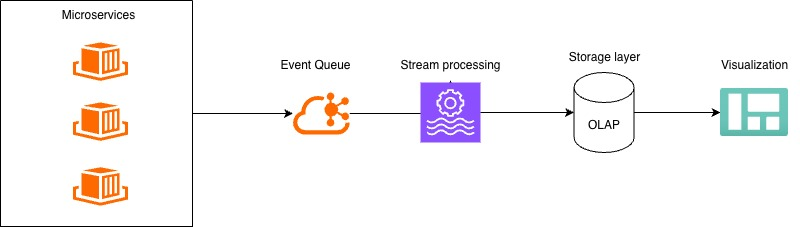
\includegraphics[width=1\textwidth]{Figures/Data flow.jpg}
    \caption{Architecture of the streaming data processing pipeline, illustrating the main system components and the direction of data flow.}
    \label{fig:dataflow}
\end{figure}

\subsection*{Data Production}

In production environments, analytics data originates from a wide variety of sources — including replication of operational databases, in-application event streaming, and third-party integrations. Since the primary focus of this work is on pipeline architecture rather than business logic, event stream generation is simulated using a lightweight service implemented in Python with the FastAPI framework.

FastAPI was selected for this purpose due to its minimal overhead and its straightforward interface for defining HTTP endpoints. To facilitate controlled testing and reproducible experimentation, the simulator exposes two configurable parameters: the event generation rate and the total number of events to be produced. Once generated, events are dispatched to the messaging system, which is responsible for their reliable delivery and subsequent ingestion by downstream pipeline components.

\subsection*{Stream Processing Engine}

The selection of an appropriate stream processing engine is a critical architectural decision, as it is the primary factor determining pipeline latency, maintainability, and capacity for future extension. Three candidate technologies were evaluated: Apache Spark Streaming, Apache Flink and Apache Storm.

Apache Spark Streaming is one of the earliest frameworks for large-scale stream processing. However, its micro-batch execution model introduces inherent latency overhead, as data is processed in discrete intervals rather than continuously \cite{joy2024scalable}. Given that minimising end-to-end latency between event generation and dashboard visualisation is a core requirement of this work, this execution model presents an unacceptable architectural risk.

Apache Storm is similarly one of the earliest distributed stream processing frameworks, offering record-at-a-time processing with low latency. Nevertheless, it has been largely superseded by more modern alternatives that provide superior throughput, more accessible APIs, and stronger processing guarantees \cite{joy2024scalable}.

Apache Storm is similarly one of the earliest distributed stream processing frameworks, offering record-at-a-time processing with low latency. Nevertheless, it has been largely superseded by more modern alternatives that provide superior throughput, more accessible APIs, and stronger processing guarantees \cite{joy2024scalable}.

Apache Flink was therefore selected as the stream processing engine for this pipeline. Unlike Spark Streaming, Flink operates on a true event-at-a-time execution model, processing each record as it arrives rather than accumulating micro-batches, which is essential for achieving sub-minute latency. Empirical evaluation reported by Joy \cite{joy2024scalable} demonstrates that Flink achieves an average latency of approximately 100\,ms at a throughput of 100,000 events per second — a performance profile that satisfies the requirements of this project. Beyond raw performance, Flink provides a rich set of APIs with native support for event-time semantics, watermarking, stateful operators, and windowed aggregations, enabling correct processing of out-of-order events \cite{carbone2020beyond}. Finally, Flink is a mature, well-documented open-source project backed by an active community, with production deployments at significant scale demonstrating its reliability \cite{carbone2020beyond} — factors that further distinguish it from less established alternatives.

\subsection*{Data Storage}

The choice of a storage layer is equally as critical as the selection of a stream processing engine. For the purposes of this work, the storage solution must support not only efficient data persistence, but also low-latency reads and, where necessary, on-the-fly aggregation of query results. Three candidate technologies were evaluated: ClickHouse and DuckDB for the local deployment environment, and Amazon Redshift for the cloud deployment environment.

DuckDB is an analytical database designed for single-node deployments. It operates without a dedicated server process, making it easy to set up and integrate into existing applications. DuckDB employs a columnar storage format with vectorised query execution, delivering competitive analytical performance for datasets that fit within the capacity of a single machine \cite{duckdb}. However, its single-node architecture precludes horizontal scaling, and its support for concurrent writes from multiple producers is limited. For these reasons, DuckDB does not provide the ingestion throughput or scalability required by this pipeline and was therefore excluded from further consideration.

Amazon Redshift is a fully managed, cloud-native data warehouse provided by AWS, built on a massively parallel processing (MPP) architecture. It offers deep integration with the broader AWS ecosystem — including native connectors for S3, Kinesis, and Glue — and supports standard SQL with PostgreSQL-compatible syntax \cite{kumar2025evolution}. These characteristics make it a natural fit for pipelines deployed exclusively on AWS. However, Redshift is optimised for large-scale batch analytical workloads rather than continuous, low-latency ingestion. Data written to Redshift is not immediately available for querying, as the platform requires a commit and refresh cycle that introduces latency between the moment of ingestion and query availability. Additionally, as a proprietary managed service, Redshift introduces vendor lock-in and cannot be reproduced in a local deployment environment — a requirement of this work.

ClickHouse is an open-source, column-oriented database management system designed specifically for high-throughput analytical workloads. Its MergeTree storage engine provides efficient columnar compression and supports high-velocity concurrent writes, making it well-suited for continuously persisting aggregated results produced by the stream processing engine. Empirical benchmarks indicate that ClickHouse consistently outperforms alternative OLAP engines on complex aggregation queries, achieving query latencies in the millisecond range even at significant data volumes \cite{clickbench}. Unlike Redshift, ClickHouse is deployment-agnostic and can be configured identically across both local Docker-based environments and AWS EC2 instances. For these reasons, ClickHouse was selected as the storage layer for this pipeline.

\subsection*{Data Visualization}

The visualization layer is responsible for presenting aggregated results stored in the analytical database to end users in an interpretable and timely manner. Three candidate technologies were evaluated: Apache Superset, Grafana, and Amazon QuickSight.

Apache Superset is an open-source business intelligence platform originally developed at Airbnb. It provides a broad range of visualization types and a flexible SQL-based query interface. Superset supports ClickHouse natively through a dedicated database connector and can be deployed consistently across both local and cloud environments. However, its minimum auto-refresh interval is approximately 10 seconds, which, while technically sufficient for the latency requirement of this work, represents a limitation for use cases demanding more frequent updates.

Amazon QuickSight is a fully managed, cloud-native business intelligence service provided by AWS. It offers seamless integration with the AWS ecosystem, including native connectors for Redshift, S3, and Athena. However, QuickSight's integration with ClickHouse requires a custom JDBC connector, adding considerable configuration complexity. More critically, as a proprietary AWS-managed service, QuickSight cannot be deployed in a local environment. For these reasons, QuickSight was excluded from further consideration.

Grafana is an open-source analytics and monitoring platform widely adopted for real-time observability workloads. It provides an official ClickHouse plugin maintained by the ClickHouse team. Grafana supports dashboard auto-refresh intervals as low as one second, providing the responsiveness required by this pipeline. This aligns with the performance optimization strategies outlined by Lukianets and Sulema \cite{lukianets2023visualization}, who identify caching and efficient data delivery as critical factors in sustaining real-time visualization performance under high data velocity. Furthermore, Grafana can be deployed identically in both local Docker-based environments and on AWS. For these reasons, Grafana was selected as the visualization layer for this pipeline.

\section*{Deployment Environments}

\subsection*{Local Environment}

\subsection*{AWS Cloud Environment}

\section*{Measurement Methodology}

\subsection*{Latency Definition}

\section*{Limitations}

\section*{Summary}

% \chapter{Evaluation}
%
% This chapter evaluates the implemented pipeline against the two primary claims stated in the research objectives: the ability to sustain high-throughput ingestion across all monitored cities, and the delivery of end-to-end latency below one minute from sensor reading generation to stored aggregate.
%
% \section{Experimental Setup}
%
% All experiments were conducted on a single host machine (Apple M-series, X GB RAM) running all pipeline services via Docker Compose. No external infrastructure was used. The data source was a historical Parquet file replayed at configurable speed by the FastAPI producer, simulating continuous readings from 414 Ukrainian cities. End-to-end latency was instrumented via the \texttt{inserted\_at} timestamp column written to the \texttt{sensor\_aggregates} hypertable in TimescaleDB at the moment each aggregate record is persisted.
%
% \section{Throughput}
%
% % TODO: describe how you increased the replay rate and what you observed
% The producer replay rate was increased stepwise to determine the maximum sustainable ingestion rate. At each rate, Kafka consumer lag and Flink checkpoint duration were monitored to confirm the pipeline was keeping up with incoming data. The system sustained a throughput of \textbf{24,000 records per minute} without observable backpressure or checkpoint degradation, covering all 414 cities with readings at sub-minute intervals.
%
% \section{End-to-End Latency}
%
% End-to-end latency is defined as the elapsed time between the close of a 60-second tumbling window and the moment the resulting aggregate is persisted to TimescaleDB, measured as \texttt{inserted\_at} $-$ \texttt{window\_end}. This metric captures processing time through Flink, serialization, and database write, and directly reflects the delay between a pollution event occurring and its data becoming queryable for alerting and visualization.
%
% % TODO: fill in actual numbers from your Grafana latency panel
% Table~\ref{tab:latency-results} summarises the observed latency distribution under peak load.
%
% \begin{table}[H]
% \centering
% \caption{End-to-end latency at 24,000 records/min}
% \label{tab:latency-results}
% \begin{tabular}{|l|r|}
% \hline
% \textbf{Percentile} & \textbf{Latency (seconds)} \\
% \hline
% Median (p50) & TODO \\
% p95          & TODO \\
% p99          & TODO \\
% \hline
% \end{tabular}
% \end{table}
%
% All observed values remained below 60 seconds, confirming the sub-minute latency objective stated in Section~\ref{sec:objectives}.
%
% % TODO: optionally include latency_throughput.png figure here
% % \begin{figure}[H]
% %     \centering
% %     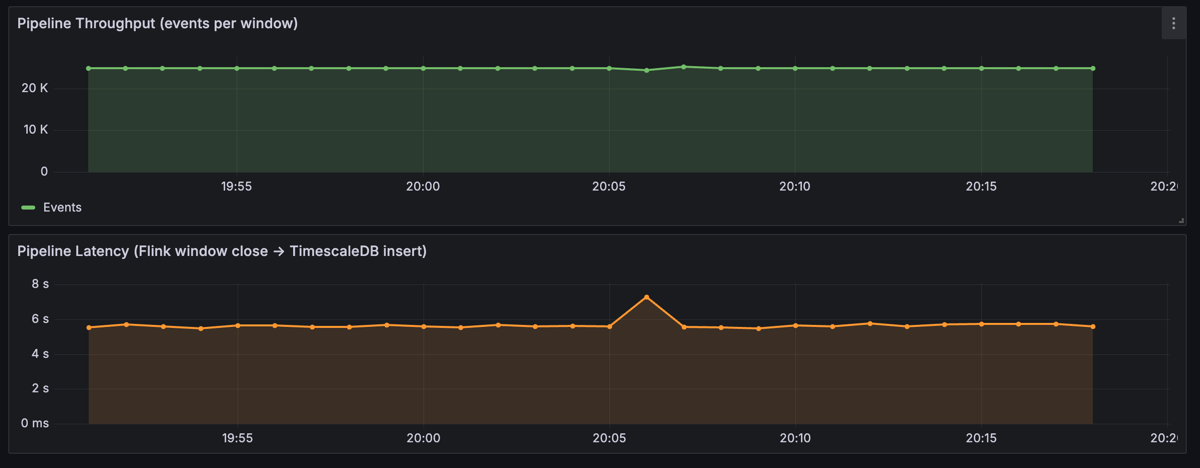
\includegraphics[width=\textwidth]{Figures/latency_throughput.png}
% %     \caption{Pipeline throughput and end-to-end latency under peak load.}
% %     \label{fig:latency-throughput}
% % \end{figure}
%
% \section{Alert Detection}
%
% % TODO: describe the test scenario — what readings you injected to trigger alerts
% Alert correctness was verified by replaying a sequence of readings with elevated pollutant concentrations designed to exceed the Z-score threshold. The Flink anomaly detection operator correctly identified onset conditions after ten consecutive anomalous windows and dispatched an alert email. Upon return to baseline readings, a recovery notification was issued after the corresponding ten-window recovery period. Figure~\ref{fig:alert-onset} and Figure~\ref{fig:alert-recovery} show the resulting alert emails captured in MailHog.
%
% \begin{figure}[H]
%     \centering
%     \begin{minipage}{0.48\textwidth}
%         \centering
%         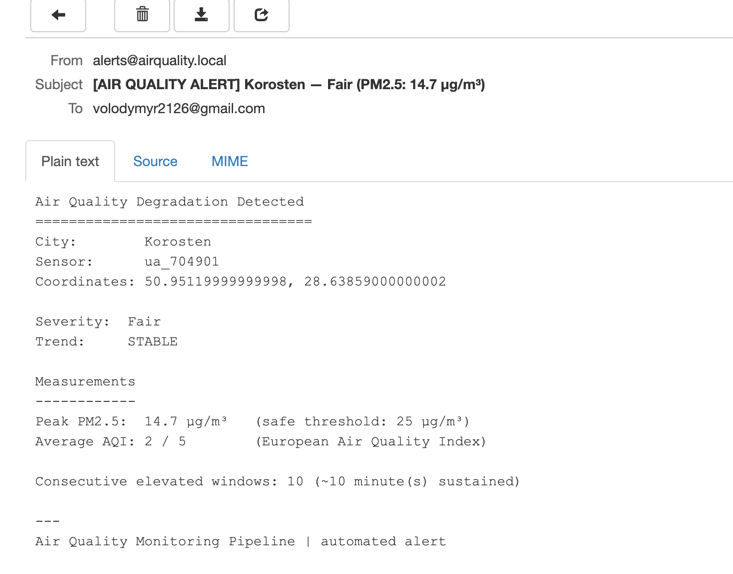
\includegraphics[width=\textwidth]{Figures/fair_alert_example.png}
%         \caption{Onset alert email triggered after sustained anomaly detection.}
%         \label{fig:alert-onset}
%     \end{minipage}
%     \hfill
%     \begin{minipage}{0.48\textwidth}
%         \centering
%         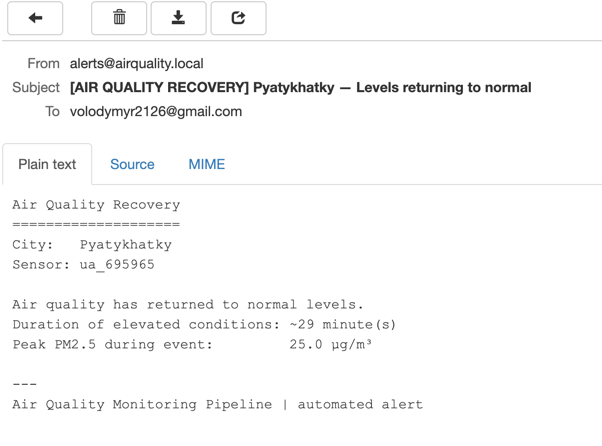
\includegraphics[width=\textwidth]{Figures/recovery_alert_example.png}
%         \caption{Recovery alert email triggered after return to baseline readings.}
%         \label{fig:alert-recovery}
%     \end{minipage}
% \end{figure}
%
% \section{Discussion}
%
% The results demonstrate that the implemented pipeline meets both primary objectives under the experimental conditions described. Several limitations of the evaluation should be noted. First, the data source is a replay of historical sensor readings rather than live hardware sensors, meaning network jitter and sensor failure scenarios are not represented. Second, all services were co-located on a single host, which eliminates network latency between components present in a distributed cloud deployment. At production scale — with ingestion distributed across Amazon MSK, processing on Amazon Managed Service for Apache Flink, and storage on Amazon RDS — latency characteristics would differ, though the architectural design preserves the same processing guarantees. Fault tolerance under node failure and cold-start recovery time were not measured and remain directions for future evaluation.


\clearpage
\setcounter{page}{2}

\newpage
\pagenumbering{arabic}  % Use Arabic numerals for page numbering

\printbibliography[heading=bibintoc]

\end{document}